%ch04

\chapter{Building Modular Attribute-Driven Transformers}
\label{ch:tango}
\label{ch04}
\mquote{All animals are equal, but some animals are more equal than the others.}{G. Orwell, Animal Farm, 1946}
\mquote{All transformations are equal, but some transformations are more equal than the others.}{(Variation)}

\noindent This chapter\footnote{This chapter shares content with references \cite{cepa.tango.ICSR8,cepa.mezini.gpce.04,cepa.mezini.hicss38,cepa.2006}.} addresses the implementation of modular attribute-driven transformers by exploring features that are specific to DSA modeling of mobile product-lines with attributes. The developed technology can be used, as well, with other attribute-driven transformations.

Using explicit attributes at the programming language level has recently been attracting a lot of attention with technologies, such as .NET attributes \cite{design.attrib} and Java 1.5 annotations \cite{www.java.attrib.04}, and also with specialized tools, such as xDoclet \cite{www.xDoclet}\footnote{xDoclet does not work at the language level.}, used with EJB \cite{www.ejb}. However, there are currently no systematic ways for transforming attribute-driven product-line specific constructs. This often results in implementations which are not very modular and hence difficult to reuse.

\begin{figure}[ht]
%	\begin{center}
	  \xymatrix{
	  	*+[F]{\txt{Attribute Transformation \\\Sr{sec.attribute.trans}}} \ar[r] \ar[d] \ar[dr]& *+[F]{\txt{Layering Transformation Strategy  \\\Sr{sec.tango.layers}}}  \\  	
	*+[F]{\txt{Automating Transformation Concerns \\\Sr{ch04:sec:dep}}} \ar[r] \ar[d]  	 & *+[F]{\txt{Related Work \\\Sr{sec.c4.related}}} \\  	
	  *+[F]{\txt{Attribute Dependency Checker Tool \\\Sr{sec:adc}}} 	  &   \\	  	
	  }
%	\end{center}
%	\caption{Chapter Overview}
%	\label{fig:contents}
\end{figure}

\Sr{sec.attribute.trans} shows how the AST could be modeled to ease attributes transformation in mobile product-lines. The addressed domain is explored to introduce a horizontal modularization of transformers. The OO language model of MIDP \cite{www.midp-ota} is used in \sr{sec.tango.layers} to layer the transformation strategy.

Automating attribute transformation concerns using meta-attributes is addressed in \sr{ch04:sec:dep}. A specialized tool, called ADC, for checking attribute dependencies based on meta-attribute decorations, is presented in \sr{sec:adc}.

Several generative and graph transformation techniques could be used to implement attribute-driven transformers. Related transformation and automation approaches for the techniques developed in \srs{sec.attribute.trans}{ch04:sec:dep} are discussed in \sr{sec.c4.related}. 

\section{Attribute-Driven Transformations}
\label{sec.attribute.trans}

The concepts discussed in this section have been implemented as part of an attribute-driven transformation framework, called \textbf{Tango}\footnote{The name \textit{Tango} was coined in the following way: tag $\rightarrow$ tag-go $\rightarrow$ taggo $\rightarrow$ tango.}. The Tango framework is designed to quickly add attribute-based domain-specific constructs to existing object-oriented (OO) languages, by reusing the existing language functionality. Tango has evolved as a generalization of the work on the \textbf{MobCon}\footnote{Mobile Container.} Transformation Engine (MTE), to support mobile containers presented in  \kr{ch05}. Examples from Tango will be used as necessary in this section, to explain different aspects of attribute-driven transformations. A distinction will be made between the introduced concepts, which are general and could be implemented in more than one way, and the concrete Tango's specific implementation.

\subsection{AST Representation}
\label{sec.ast.tango}

The starting point for the representation of the abstract syntax tree (AST) in attribute-driven transformers will be a GAAST-like API \seec{ch03}. As the focus of this section is on attribute-driven transformers used to support mobile software product-lines, an abstraction over the AST is utilized to facilitate the transformations for this domain. 

\begin{figure}[ht]
	\begin{center}
		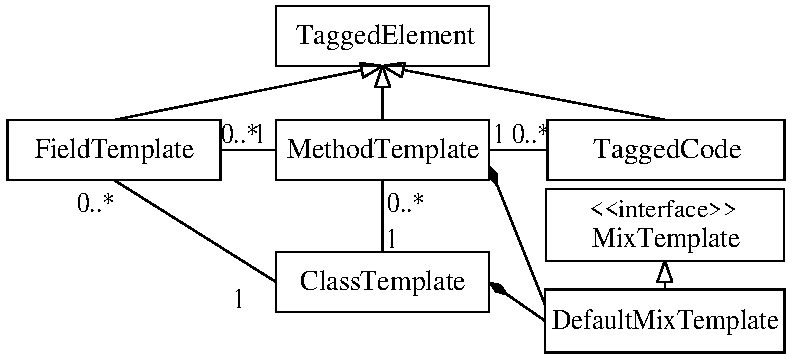
\includegraphics[width=8cm,height=!]{ch05/ct-ast2}
	\end{center}
	\caption{CT-AST API}
	\label{fig:ct-ast}
\end{figure}

Internally, the GAAST representation is organized around a class-based API called a \textit{Class Template AST (CT-AST)}, shown in \fig{fig:ct-ast}. The CT-AST API wraps the original AST of the source code \seec{ch05} and contains operations that facilitate the AST manipulation of classes and methods. For example, method bodies are represented as a list of attribute decorated \texttt{TaggedCode} elements divided into three logical blocks: begin, middle, and end (\fig{fig:method-body2}).

\begin{figure}[ht]
	\begin{center}
		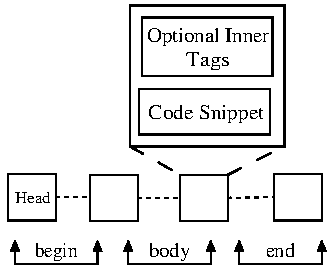
\includegraphics[width=5cm,height=!]{ch05/method-body2}
	\end{center}
	\caption{CT-AST Method Body Model}
	\label{fig:method-body2}
\end{figure}

This organization helps transformers to select code elements of interest based on attributes and to insert new code elements before or after any other code block. When an existing method is parsed in code, its method body is represented as a single code element in the middle block\footnote{All transformers of prototype for J2ME MIDP of \kr{ch05} work at the method block level.}. Each element of the CT-AST API derives from a {\tt Taggeg\-Ele\-ment} and can be decorated with one or more attributes \see{sec.inner.tags}. Support for merging different class templates is provided using a {\tt De\-fault\-Mix\-Tem\-pla\-te} class \see{sec.workflow}.

\begin{figure}[ht]
	\centering
	\begin{minipage}[b]{12cm}
	\begin{center}	
\begin{scriptsize}
\begin{lstlisting}[numbers=left,language=XML,frame=leftline]{}
<!ELEMENT methodbody (startblock?, middleblock?, endblock?) >
<!ELEMENT startblock (taggedcode)+ >
<!ELEMENT middleblock (taggedcode)+ >
<!ELEMENT endblock (taggedcode)+ >
<!ELEMENT taggedcode (tags?, code) >
<!ATTLIST taggedcode name CDATA #IMPLIED >
		\end{lstlisting}
		\end{scriptsize}
	\end{center}
	\caption{Tango's Internal Model of the Method Body}
	\label{c4f:tango.model}
	\end{minipage}	
\end{figure}

Internally, Tango works with an XML \cite{skonnardetal.01} representation of the CT-AST and expects the input to be converted to XML. For example, \fig{c4f:tango.model} shows how the method body is modeled in Tango as XML DTD. This enables more flexibility for processing code originating from more than one language, that conforms to the CT-AST meta-model. The internal XML representation externalizes the AST parsing outside Tango. The AST parsing can be done with any parsing or meta-programming tool\footnote{\Kr{ch05} explains how the real AST for J2ME MIDP is obtained.}.

\begin{figure}[ht]
		\centering
		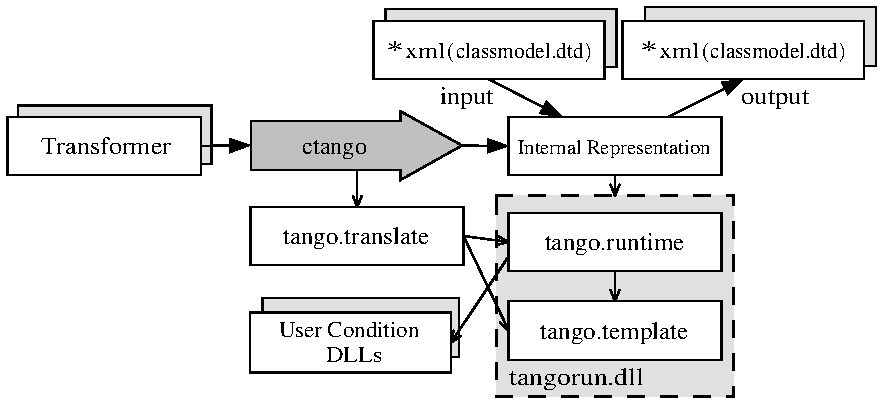
\includegraphics[width=10cm,height=!]{ch04/tango}
	\caption{Tango Framework}
	\label{fig:tango}
\end{figure}

The high-level organization of Tango is shown in \fig{fig:tango}. The usage of the XML representation is implicit in Tango. Tango supports a set of CT-AST classes around XML (part of \textit{tango.template} namespace in \fig{fig:tango}) similar to those in \fig{fig:method-body2}, that are used by the transformers. The node selection operations of Tango are internally mapped to XML queries using XPATH \cite{url.xpath}. The Tango processor (ctango) invokes the Tango run-time to process the input code encoded in the Tango's XML format. The transformation functionality is specified as input to the Tango processor. This functionality is first mapped onto the internal Tango representation in XML (\textit{tango.translate} namespace). The Tango processor invokes the Tango run-time (the transformation engine) that maps the input code to the output code based on the transformation logic\footnote{Custom user condition DLLs are explained in \sr{sec.tango.layers}.}.


\subsection{Class Transformations}
\label{attrib.trans}

Classes annotated with attributes serve as input units for attribute-driven transformers. \fig{fig:ch04tg} shows that an attribute annotated class can be transformed in two ways. A new class can be created, or the class can be modified in place\footnote{More than a single new class could be created. In-place class transformation and creation of the new classes can also be combined (see equation~\ref{eq.main}).}. The exact transformation will depend on the semantics that attributes carry and the specific invasive technology used.

\begin{figure}[ht]
		\centering
		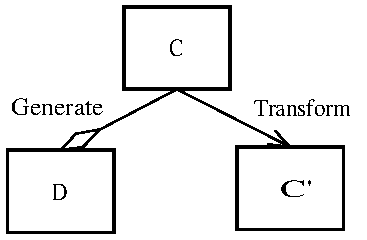
\includegraphics[width=4cm,height=!]{ch02/transgen}
	\caption{Transformation and Generation}
	\label{fig:ch04tg}
\end{figure}

\begin{itemize}
\item \textit{Creating a new class.} A class $C$ annotated with attributes is processed with a transformer $T$, giving a new class $D$, such that $D$ = $T(C)$. The $D$ class is called an adapter \cite{dpatterns}. The original class $C$ does not change. The adapter $D$ contains the additional functionality introduced by $T$, and forwards the messages as necessary to the original class $C$. Both, $D$ and $C$ must be present in the system. Another way to implement $D$ is based on the template pattern \cite{dpatterns}. In this view, $D$ is the result of the template $T$, where the specialization C is applied: $D$ = $T<C>$. The class $D$ is \textit{generated} based on the class $C$.

The implementation of $T$ requires that the $C$'s implementation is independent of the intended attribute semantics. This means that $C$ should be successfully compiled ignoring the attributes. This transformation in not possible for most attribute-based DSA. To maximize automation, attributes are used to introduce changes in the code before compilation.

The $D$ class can either be obtained before (or during) compilation, or at run-time using reflection when supported. For example, .NET saves structural attributes into the compiled binary. At run-time, annotations can be accessed using reflection. In .NET languages, rather than using the component $C$ directly, the implementation of $D$ can use reflection over the original component $C$\footnote{It becomes a bottleneck if a lot of reflection code is written every-time, unless an adapter pattern \cite{dpatterns} is used.}. Alternatively, $D$ can be generated before compilation using the .NET \textit{CodeDom API} \cite{cdom} over the component $C$'s source code. The adapter $D$ could also be changed dynamically resulting in some form of dynamic AOP \cite{kiczalesetal.97}\footnote{In this case, the rest of the program should be aware of the adapter $D$ and use it instead of using the class $C$ directly which may not be always acceptable.}.

\item \textit{In-place class modification.} The annotated class implementation is dependent on the semantics of the tags. $C$ could not be compiled directly without applying some transformation (add / remove code) to it. In this case, the attribute-based transformer $T$ gives a new class $C'$, such that $C'$ = $T(C)$. Only the class $C'$ must be present afterward in the system. The class $C$ is \textit{transformed} into the class $C'$.

In-place class modification supports invasive changes that need to be applied before compilation. These changes are needed to support attribute-based DSA, and when the original system is not designed with transformation in mind (and makes direct use of $C$, rather than through a new component $D$).
In-place class transformations are usually applied to source code, because generally the class $C$ can not be compiled directly.
\end{itemize}

\noindent The symbol $\Gamma$ will be used to stand for both $D$ and $C'$, when it not necessary to distinguish the two cases, that is $\Gamma$ = $T(C)$. If  $C$'s implementation supports non-invasive transformations, then $\Gamma$ could be either $D$ or $C'$ since both are possible, otherwise it is $C'$. $\Gamma$ is the result of the transformation process, that is, $\Gamma$ is the final implementation of $C$. $\Gamma$'s implementation is identified by the tuple $<T, C>$. The motivation to split $\Gamma$'s implementation is that the same transformer $T$ can be used for any class $C$ decorated with attributes that drive the $T$ transformation. This way, an entire set of classes $\{\Gamma\}$ is parameterized based on an implementation set $\{C\}$. $T$ can be seen as an implementation template, parameterized by $C$. The functionality of $T$ does not need to be repeated in every element of $\{\Gamma\}$.

Additional specialization parameters can be specified as a parameter vector $\Pi$ to T, that is $\Gamma$ = $T(\Pi, C)$. Parameters offer a convenient way to parameterize $T$ independently of the implementation of $\{C\}$. The representation $\Gamma$ = $T(\Pi, C)$ is very general. It can be implemented in various ways, e.g., using high-order functions \cite{mozart.04}, or generics (templates) \cite{generative.00}, depending on the hosting language technology. The focus will be on implementing $T$ for attribute-driven transformers, which usually apply in-place class modifications.

Implementation of attribute-based transformers is usually difficult, because more than a single attribute needs to be processed as part of a complex context. Usually an attribute-driven transformer $T$ takes as input a set of classes $\{C\}$ decorated with several attributes $\{\tau(\pi)\}$, where $\pi$ are the parameters of a single attribute $\tau$. Thus, an attribute transformer $T$ can be defined as a transformation function by the equation~\ref{eq.main}:

\begin{equation}
\{\Gamma\} = T(\{\tau(\pi)\}, \{C\})
\label{eq.main}
\end{equation}

\noindent The transformer $T$ in equation~\ref{eq.main} transforms a set of input classes $\{C\}$ decorated with a set of attributes $\{\tau(\pi)\}$ into a set of output classes $\{\Gamma\}$. The attribute set $\{\tau(\pi)\}$ is the \textit{coupling set} between $T$'s implementation and $\{C\}$.
%
The implementation of $C$ needs to be accessed inside the implementation of $T$, in order to be able to reason about it. Only the case when $C$ is source code will be considered in this chapter. Other transformation based on the same technology can be used for other representations of $C$, e.g., in the Java bytecode representation, if the possibility to access and manipulate similar entities exists in those other representations.

\subsection{Mapping Transformation Logic to Attribute Families}
\label{sec.tango.domain}

\Sr{attribute.families} explained how attribute families can be used as a variability mechanism for product-lines. Attribute families could also help to logically organize attribute-based DSA transformations. They drive the first modularization of $T$ in equation~\ref{eq.main}.

Each family of attributes can be processed by a single transformation unit specialized for that family. Formally, the entire attribute set $\{\tau(\pi)\}$ is split in a finite series of disjoint subsets $\phi_i$, corresponding to each attribute family $i$ in a domain of interest. The transformation function $T$ in equation~\ref{eq.main} can be then expressed as a composition of transformers $\Phi_i$ corresponding to the $N$ attribute families:

\begin{equation}
\{\Gamma\} = \Phi_1 \circ \dots \circ \Phi_N(\{\tau(\pi)\}, \{C\}) 
= \Phi_1(\phi_1, \{C\}) \circ \dots \circ \Phi_N(\phi_N, \{C\})
\label{eq.compose}
\end{equation}

All individual family transformers have access to all classes passed as input to $T$ and select the ones of interests based on their specific attributes $\phi_i$. The decomposition of each transformer $\Phi_i$ could be done similarly, if needed, based on attribute sub-families. The $\Phi_i$ transformers of individual attribute families can be organized as plug-ins of a generic attribute-driven transformation framework \seec{ch05}.

\subsection{Controlling Composition Semantics with Inner Tags}
\label{sec.inner.tags}

A side-effect of the equation~\ref{eq.compose} is that it removes the global transformation state that was preserved in $T$ (equation~\ref{eq.main}). There is no global way to maintain information about the overall transformation process. Results of previous computations should be explicitly passed to the next transformer in the chain. This can be done by means of additional parameters passed to each $\Phi_i$, or by encoding the information to pass in the transformed classes that result from the input $\{C\}$. Each transformer $\Phi_i(\phi_i, \{C_i\})$ needs to re-parse the information of the previous transformer $\{C_i\} = \Phi_{i - 1}(\phi_{i - 1}, \{C_{i - 1}\})$. Reprocessing the AST can be avoided, if the information that needs to be passed between the transformers is also encoded as attributes. Now, each transformer has the form $\Phi_i(\phi_i, I_i, \{C_i\})$, where $I_i$ are the additional attributes expected to be found in $\{C_i\}$ before the $\phi_i$-driven transformation can be applied. The $I_i$ attributes do not represent directly domain-level concepts as the $\phi_i$ do. When present, the $I_i$ attributes only help with the transformation concerns. The output $C'_i$ of each transformer $\Phi_i$ is decorated with a set of attributes $O_i$ made up of a combination of the unprocessed explicit attributes, and the $I_{i+1}$ phase attributes added during the $\Phi_i$ transformation:

\begin{equation}
(O_i, \{C'_i\}) = \Phi_i(\phi_i, I_i, \{C_i\})
\label{eq.trans}
\end{equation}

In Tango, the $I_i$ attributes are known as \textit{inner tags} (or attributes). Tango treats the inner tags as a natural extension of the explicit attributes, that enable a declarative transformer composition. Inner tags are used only in the inner operations of attribute-driven transformers and offer a convenient means for specifying the \textit{coupling sets} between the composed transformers, by removing the need to reinterpret the code. Inner tags are similar to ASF+SDF \cite{asfsdf.02} \textit{placeholders} for saving intermediate results. In Tango, the inner tags offer a uniform model to controll custom semantics, that is integrated uniformly with the remainder of attribute-driven transformer operations. Transformers deal with the inner tags in the same way they process the explicit attributes. All Tango's basic edit operations can specify inner tags to decorate the entities that they modify. 

\begin{figure}[ht]
		\centering
		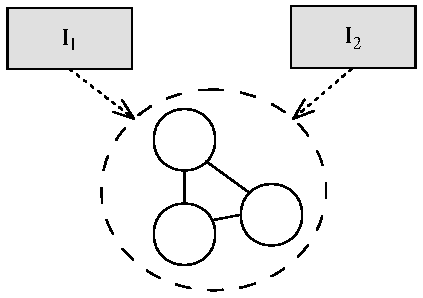
\includegraphics[width=5cm,height=!]{ch04/it-node}
	\caption{AST Node Grouping and Labeling with Inner Tags}
	\label{fig:it-node}
\end{figure}

While inner tags place transformer interaction semantics, the alternative is to reprocess the AST in each transformer, to check whether it fulfills a given condition. Using inner tags does not grow transformer coupling (it remains the same). Inner tags only make the coupling declarative, avoiding AST reprocessing. Logically, the inner tags are used to create arbitrary graph node sets \cite{mens.99}, which may not correspond directly to the generalized AST graph nesting structure as shown in \fig{fig:it-node}. A group of AST nodes is decorated with same inner tags to form a single logical node unit. Inner tags also help to associate more than one label with a node (group) as in \fig{fig:it-node}, in order to select the node in more than one logical set.

\begin{figure}[ht]
		\centering
		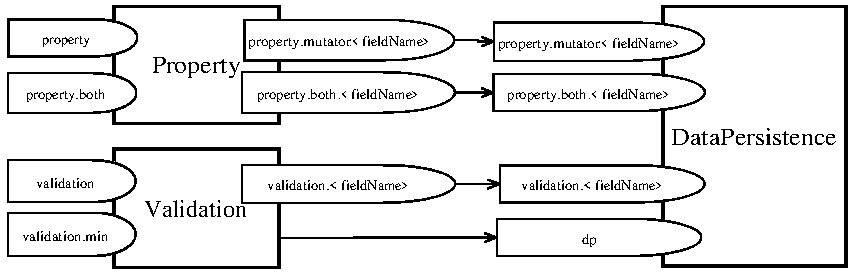
\includegraphics[width=12cm,height=!]{ch04/tcomp}
	\caption{Transformer Composition Based on Tags}
	\label{fig:tcomp}
\end{figure}

Consider again the attribute-driven transformation example of \fig{fig:input}, presented in \sr{attribute.families}.
\fig{fig:tcomp} shows a possible combination of the three attribute-driven transformers, namely, \texttt{Pro\-per\-ty}, \texttt{Va\-li\-da\-tion} and \texttt{Da\-ta\-Per\-si\-ste\-nce} for processing the code of the example in \fig{fig:input}. The exact combination order may change in a particular implementation.  In this example, the \texttt{Pro\-per\-ty} transformer  expects the input unit(s) to be decorated with attributes \texttt{property} and \texttt{property.both}. The \texttt{Pro\-per\-ty} transformer decorates its output, which is made of the added property methods, e.g., \texttt{set\-Sco\-re()}, and their corresponding fields, e.g., \texttt{score}, with a \texttt{pro\-per\-ty.mu\-ta\-tor.$<$field\-Na\-me$>$} inner tag (among the other tags). The \texttt{$<$field\-Na\-me$>$} in \fig{fig:tcomp}  stands for the actual field name, e.g., \texttt{score}. The actual value is expanded during the transformation process.

The \texttt{Da\-ta\-Per\-si\-ste\-nce} transformer combines the output of the two previous transformers.  \texttt{Da\-ta\-Per\-si\-ste\-nce} requires that the AST, it works upon, is decorated among the others with the (inner) tags \texttt{prope\-rty.both.$<$field\-Na\-me$>$} and \texttt{va\-li\-da\-tion.$<$field\-Na\-me$>$} to be able to read, modify, and validate the field data inside the persistence code that it adds. \texttt{Da\-ta\-Per\-si\-ste\-nce} treats the inner tags, e.g., \texttt{pro\-per\-ty.mu\-ta\-tor.$<$field\-Na\-me$>$}, in the same way it treats explicit attributes, e.g.,  \texttt{dp}, and cannot distinguish between the two.

\subsection{The Transformation Workflow}
\label{sec.workflow}

For the transformation of the equation~\ref{eq.compose} to be applicable in practice, a partial order over $\Phi_i$ should be found. The partial order of $\Phi_i$ depends (a) on the domain assets that $\Phi_i$ models, expressed by the attribute set $\phi_i$ and (b) on the details of the $\Phi_i$ implementation, expressed by the attribute set $I_i$. The implementation order is accidental, and the $I_i$ will depend on the order placed upon $\phi_i$. Because the transformers $\Phi_i$ model domain concerns, they can be named according to the concerns they address ($\Phi_i\rightarrow name$). The names of the $\Phi_i$ transformers can be used by the developers to define a partial order over $\Phi_i$. The process can be partially automated by specifying for each addressed domain concern, what other concerns need to be processed before and after it, as $\Phi_i\{before\} \{after\}$ lists. The elements of before and after lists are made of the $\Phi_i$ transformer names, or of special quantifier symbols, e.g., \textit{all} or \textit{any}. These local dependency relations are processed automatically to build the total $\Phi_i$ dependency graph, as shown in the example of \fig{fig.dependency}. Encoding the dependency relations locally in each transformer, rather than globally, is preferable, because the dependency relations depend on the particular implementation of the $\Phi_i$. The local encoding of dependencies frees the developers from having to build manually the total dependency graph.

\begin{figure}[ht]
		\centering
		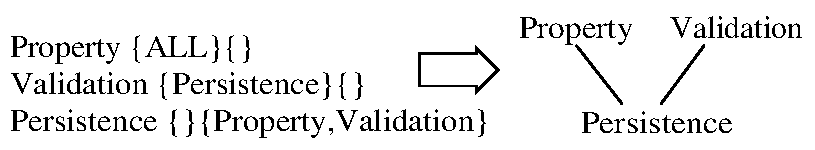
\includegraphics[width=8cm,height=!]{ch04/dependency}
	\caption{Resolving Dependencies}
	\label{fig.dependency}
\end{figure}
 
The dependency graph defines the transformation workflow. The developers can modify the automatically generated dependency graph manually to resolve any conflicts, on a case by case basis. A minimal workflow language is supported in Tango for this purpose. The Tango's workflow syntax is made up of (a) class variables ('\$') that can point to the processed classes, (b) constructors that create empty or initialized class variables, and operations to save them back to source files, (c) an operation to assign (deep copy) the class variables ('='), and (d) two composition operators:  the sequential composition (',') (which is equivalent to the function '()' operator) and the try operator ('$|$') that is similar to an 'if ... else' construct. A transformer in Tango, either succeeds or fails.

For example, the workflow order of the transformers of \fig{fig:tcomp} can be specified as \texttt{\$CT = Property, Validation, Persistence;} which is equivalent to \texttt{\$CT = Per\-si\-ste\-nce(Va\-li\-da\-tion(Pro\-pe\-rty(\$CT)));}. Actually both notations are supported. For the MIDP domain concerns addressed in this book, e.g., data \texttt{Per\-si\-sten\-ce}, it makes no sense to apply the transformations continuously to a class. For this reason, Tango, currently, does not define loops, or other more sophisticated workflow operations.

Once the dependency graph, based on the domain concerns, is in place, the inner tags are used inside the transformer implementations to coordinate the control flow inside the individual transformers. Sometimes \textit{transformation adapters} need to be created to process the input, so the code has the form and the inner tags expected by an existing transformer. The equation~\ref{eq.compose} leads to a sequential evaluation of transformers. However, based on the domain dependency graph, some of the $\Phi_i$ transformers could be orthogonal to the others and the parallelism ('$||$') could be explored: 

\begin{equation}
\{\Gamma\} = (\bigcirc, | |) \Phi_i(\phi_i, I_i, \{C_i\}), i \in {1,N}
\label{eq.par}
\end{equation}

For example, in \fig{fig:tcomp} the input AST for the \texttt{Da\-ta\-Per\-si\-ste\-nce} comes from two other transformers that could work in parallel \texttt{Pro\-per\-ty} and \texttt{Va\-li\-da\-tion}. The \texttt{Da\-ta\-Per\-si\-ste\-nce} transformer does not need to reevaluate the AST. It only checks for the required attributes. In this case \texttt{Da\-ta\-Per\-si\-ste\-nce} mixes also the output of \texttt{Pro\-per\-ty} and \texttt{Va\-li\-da\-tion} transformers. In this case, \texttt{Pro\-per\-ty} and \texttt{Va\-li\-da\-tion} could also be seen as adapters of the original AST, to make it suitable for further processing by the transformer \texttt{Da\-ta\-Per\-si\-ste\-nce}. All the composition semantics are represented as attribute names (labels) in \fig{fig:tcomp}.

Because of the parallelism, different versions of the same class could be present during the transformation, as in the case with the classes output by the \texttt{Pro\-per\-ty} and \texttt{Va\-li\-da\-tion} transformers. Because of the orthogonality of parallel transformers, these classes need to be merged. A default merge operation that returns the union of the members of two classes, and the union of corresponding method code blocks \see{sec.ast.tango} is provided in MobCon \see{sec.mc.wf}. More complicated class merging need to be coded manually inside a transformer. Tango generalizes the merging concept by allowing any combination of classes to be merged at once inside a transformer. This enables a uniform composition of the transformers, unlike other systems, e.g., JMangler \cite{jmangler}, that make a distinction between individual transformers and mergers. While Tango evaluates all transformers sequentially, threading and synchronization could be implemented automatically if needed, based on the data flow \cite{mozart.04} graph on the $\Phi_i$ transformer boundaries.   
 
\subsection{Layering the Transformation Strategy}
\label{sec.tango.layers}

Up to now, only the knowledge of the domain assets is used to enable a \textit{horizontal} modularization of the attribute-driven transformers \see{sec.tango.domain} and to define the transformation workflow \see{sec.workflow}. It is also possible to explore the features of the supported language meta-model to enable a \textit{vertical} modularization of the transformers. Tango uses a common OO meta-model based on classes, fields, methods, and method blocks. This hardwired OO meta-model is enough to support the transformations that mobile containers introduce in an OO mobile product-line \seec{ch05}. The specific features of the language meta-model have been used in the past to create customized solutions for specific sets of languages. For example, denotational semantics \cite{sem.99,apld.96} explore the features of procedural languages, in order to provide a specialized model for expressing and verifying language semantics, which applies better to procedural languages than the generic operational, or axiomatic semantics \cite{sem.99}.

\begin{figure}[ht]
		\centering
		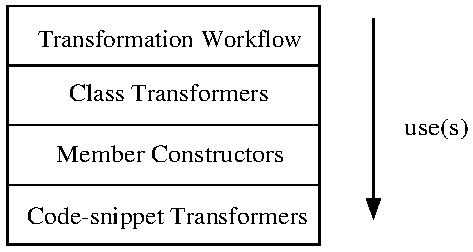
\includegraphics[width=6cm,height=!]{ch04/layers}
	\caption{Tango Framework Layers}
	\label{fig:layers}
\end{figure}

The structural information of the hardwired common OO meta-model can be used to structure the transformation \textit{strategy} \cite{stratego.01} in layers, corresponding to the nesting of the structural elements in the OO meta-model. Layering enables reasoning at different levels of abstraction about the transformation strategy, and enhances the reuse of the low-layer modules in more than one transformer. The attribute-transformers in Tango are organized in several hierarchical layers, shown in \fig{fig:layers}. The \textit{transformers workflow layer} was already discussed in \sr{sec.workflow}, the \textit{class transformers layer} ($T_c$) defines operations applied to classes, the \textit{member constructors layer} ($T_m$) defines operations applied to fields and methods, whereas the \textit{code snippets layer} ($T_s$) helps to manipulate the code templates that are used inside the method blocks. The transformer $\Phi_i$ of equation~\ref{eq.trans} can be written as:

\begin{equation}
\Phi_i(\phi_i, I_i, \{C\}) = T_{c_i}(\{C\},T_{m_i}(\{C_{members}\}, T_{s_i}(\{members_{code\_blocks}\}) ) )
\label{eq.layers}
\end{equation}

The information about $\phi_i$ and $I_i$ is distributed as needed between the transformers of each layer. The classes from \{C\} to be processed in $T_{ci}$ are again selected based on the $\phi_i$ and the $I_i$ attributes, as in $\Phi_i$. Layering is possible in Tango because the OO meta-model is hardwired, so the nesting of the structural elements is completely known. An open meta-model cannot be layered clearly with declarative constructs specialized for its elements. 

Tango enforces layering using special syntax. Every attribute-driven transformer implemented in Tango has to be modularized to conform to the layering of \fig{fig:layers}. Each layer uses the elements of the successive lower layer, but cannot create elements of the upper layer. For example, class templates are only created in the workflow layer. The class transformer layer can only modify the class templates, but cannot create new ones. To find out which class templates take part into a transformation, only the workflow layer needs to be examined. Similarly, member constructors are used in the class transformers layer only. Finally, code snippets are used only by the member constructors.

\begin{figure}[ht]
	\begin{center}
	\begin{minipage}[t]{10cm}
		\begin{scriptsize}
		\begin{lstlisting}[numbers=left,language=Java,frame=leftline]{}
transformer Property(~ct) {
precondition {
    if(not check(~ct, tags(["property"])))
         noapply;
}
action {
    $fields = select(~ct, FIELDS, tags(["property.*"]);
    if(check($fields, empty())) error;
    iterator($field in $fields) {
        if(check($field, tags(["property.accessor"])
            or tags(["property.both"])))
            add(~ct, METHOD, GetMethod($field),
                [tag(<"property.accessor", $field.name>)]);
        else if(check($field, tags(["property.mutator"])
            or tags(["property.both"])))
            add(~ct, METHOD, SetMethod($field),
                [tag(<"property.mutator.", $field.name>)]);
    }
}
return ~ct; // optional the first argument is returned
}		
		\end{lstlisting}
		\end{scriptsize}
		\end{minipage}
	\end{center}
	\caption{The Property Class Transformer Implementation}
	\label{fig:property}
\end{figure}

To understand how vertical layering is implemented beyond the workflow level, consider how the \textit{Property} attribute family transformer for the \textit{GameScore} example of \fig{fig:input} can be implemented. \fig{fig:property} shows the complete implementation of the \textit{Property} transformer (class transformers level) in Tango.
Each \textbf{class level transformer} operates in one or more class template variables, passed to it as arguments by the workflow layer, e.g., the \verb ~ ct at line 1 of the code shown in \fig{fig:property}. The class level transformers cannot create new class templates. If new class templates need to be created, this has to be done at the workflow level. 

A class level transformer in Tango has two main parts: an optional \textit{precondition} part (lines 2 - 5) and an \textit{action} part (lines 6 - 19) (\fig{fig:property}). The optional precondition section is used to apply some quick checks on the input, in order to decide whether the transformation can be applied or not. Only non-edit operations are allowed in the precondition section. Tango preconditions are \textit{optimistic}. The action part can apply more specific checks, and the transformer may still fail as a consequence of a failed condition in the action part, even thought the preconditions succeeded. The precondition section is only aimed at being able to quickly determine the attribute family, or the main inner tag families, supported by the class transformer. Preconditions are not performance optimizations rather, they give a clue about the attribute family semantics addressed by the transformer. Preconditions remove the need to consult the more complex action section, when only a high-level view inside the functionality of a class transformer is needed. The \textit{noapply} operator (line 4) tells the Tango workflow that this transformer cannot be applied. If a transformer fails to apply, the control is returned to the workflow. Theoretically, a pre-condition and a post-condition  can be defined for any graph rewriting operation \cite{mens.99}, but in practice, it is cumbersome to enumerate them for each operation (post-conditions can be written as preconditions \cite{mens.99}), so only important checks are applied in the preconditions part in Tango.

The AST editing operations are allowed only in the \textit{action} part. The action part (lines 6 - 19) will modify the input class template, to add getter and setter methods for all fields decorated with an attribute belonging the \textit{property} family. The fields are selected in line 7 and stored as a list in the variable {\tt \$fields}. The generic \textit{select} operation is used to filter a set of nodes of the same type that fulfill a given condition. Only predefined types of the supported meta-model, e.g., {\tt FIELDS, ME\-THODS}, can be used. The third argument of \textit{select} is a \textit{condition}. Several predefined conditions are supported:
\begin{itemize}
\item 'tag' - filters AST nodes based on attributes,
\item 'name' - filters AST nodes based on names,
\item 'empty' - checks whether a node list is empty,
\item 'count' - checks the number of list items.
\end{itemize}

For conditions that expect string arguments, regular expressions are supported. Users can define additional custom conditions by implementing a required interface \texttt{IUser\-Con\-di\-tion} and packing the condition logic as a separate DLL placed in a predefined sub-folder. Every time the Tango's run-time finds an unknown condition name, the run-time searches whether a custom condition DLL with the same name can be found. If found, the DLL is loaded and the \texttt{IUser\-Con\-di\-tion} interface is used to invoke a generic {\tt Fil\-ter} method using reflection. Any argument list for the condition is passed to the {\tt Fil\-ter} method. The {\tt Fil\-ter} method returns a filtered list. If no such DLL is found, or an exception occurs when the DLL is invoked, an error is reported.

The \textit{check} operation in line 8 is similar to \textit{select}. It applies all the conditions passed to it as the first argument and returns a \textit{Boolean} value indicating whether conditions have succeeded or not. The individual conditions can be combined using Boolean operators: {\tt and, or, not}. The \textit{check} and \textit{select} operations pass the first argument implicitly to all conditions. This makes it easier to understand what a \textit{check} or \textit{select} statement does, given that all conditions work on the first argument of \textit{check} or \textit{select}\footnote{At the cost of a slightly slower implementation, since each condition has to re-iterate through the input list. Set operations are used to mix the results of different conditions: \texttt{and} corresponding to \textit{intersection}, \texttt{or} corresponding to \textit{union}, and \texttt{not} corresponding to set \textit{difference}. Given that \texttt{not} operation is easier to implement during iteration, the \texttt{Fil\-ter} method of the \texttt{IUser\-Condi\-tion} interface, accepts a special boolean flag indicating the \texttt{not} condition.}, and is similar to the concept of \textit{conventional interfaces} in \cite{sicp.96}\footnote{\url{http://mitpress.mit.edu/sicp/full-text/book/book-Z-H-15.html\#\%25_sec_2.2.3}}.

The iterations over the meta-model AST are divided between the \textit{check}, \textit{select}, and \textit{iterator}. The \textit{check} and \textit{select} operators do implicit iterations over \textit{finite} lists of elements (via the conditions). The \textit{iterator} operation in line 9 is used to apply an operation to all the elements of a list. The \textit{iterator} and \textit{select} could be a single operation, however, it makes sense to separate these operations in cases when lists, other than those returned by \textit{select}, are processed. 

The \textit{add} operation (lines 12 and 16) is an example of an edit operation. It adds a meta-element to the class template given as its first argument. The {\tt Get\-Me\-thod} and {\tt Set\-Me\-thod} are member constructors. All supported edit operations in the class transformers layer, i.e., \textit{add}, \textit{delete} and \textit{modify}, work upon class templates and use member constructors of the next lower layer. In the example of \fig{fig:property}, the \textit{add} operation also appends an inner tag to the newly added element: \texttt{[tag(<"pro\-pe\-rty.acce\-ssor", \$field.na\-me>)]}. The tag is created by the explicit attribute constructor \textit{tag}, combining the field tag type and the field name, by using the string concatenation operation \verb@<...>@. This inner tag can be used later in a \textit{select}, or \textit{check} statement of another transformer in the same way as an explicit attribute.

The \textit{add} and \textit{select} operations use a common pattern. The type of processed meta-elements is given explicitly. This improves the readability of the code (in the case of \textit{add}, the type could have been deduced from the member constructor type). An alternative would be to have distinct operation names for each meta-element type, e.g., \textit{addMethod}. This would then require to maintain the Tango parser if its supported language meta-model is customized. The modified class template is returned in line 20. %For an implementation of the two other transformers of this example consult \cite{tango.04}.

The \textbf{member constructors} layer defines the actual meta-model member implementations that are used in the class transformers layer. Class templates cannot be passed as arguments to the member constructors. Currently, Tango defines member constructors for fields, methods and tags. As explained in \sr{sec.ast.tango}, method bodies are represented as a list of attribute decorated code snippets divided into three logical blocks: begin, middle, and end (\fig{fig:method-body2}). This representation enables to quickly add or remove blocks of code to a method, without dealing directly with the AST node composition. All the changes that the attribute-based DSA for mobile containers introduce, modify the method internals at the block level only.

\begin{figure}[ht]
\begin{center}
\begin{minipage}{7cm}
\begin{scriptsize}
\begin{lstlisting}[numbers=left,language=Java,frame=leftline]{}
method ToRecord($fieldArray) {
  methodName(makeMethodName(["toRecord"]));
  methodReturn(ByteArray());
  addBody(StoreFields($fieldArray));
}
\end{lstlisting}
\end{scriptsize}
\end{minipage}
\end{center}
	\caption{Method Constructor Example}
	\label{fig:method}
\end{figure}

\fig{fig:method} shows a method member constructor \texttt{To\-Re\-cord}, that is used in the persistence transformer. The constructor expects an array of fields that will be serialized in a byte array, and returns the implementation of a method \texttt{toRecord} that takes care of the serialization. The method name for the newly created method is set in line 2, and its return type is set in line 4. The example specifies the method return type by invoking a code-snippet constructor \textit{ByteArray} (line 3). A code block is added in the middle block of the method, by using the \texttt{addBody} statement in line 4. The \texttt{addBody} invokes another code snippet constructor namely, \textit{StoreFields}, to obtain the code that implements the field serialization. The method body is produced by the code snippet constructor \textit{StoreFields} (\fig{fig:code}). The \textit{addBody} operation adds this code snippet at the end of the middle block list. No direct code is manipulated in this layer. Instead the code-snippet constructors, e.g., \textit{ByteArray} and \textit{StoreFields}, are called.

\subsection{Code-Snippet Templates}

\Sr{ch2:inv} explained that invasive techniques lead to writing more code because of the meta-level indirection of the programming model. The situation can be improved by using code templates \cite{voelter.generation,java.compost}. Attribute-based DSA modify the components they decorate. Most of the changes happen inside the method boundaries, or by adding new methods. Code templates can help (a) to reduce coding efforts inside the member constructors layer and (b) to isolate the rest of an attribute-driven transformer from the language specific details.

In Tango, the transformation abstractions are isolated from the remainder of the transformer implementation via the concept of a \textit{code snippet}\footnote{This term is borrowed from .NET CodeDom API \cite{cdom}.}, which is similar to Stratego's \cite{stratego.01} \textit{concrete syntax}. A code snippet is a source code node that Tango treats as a string. It is the only part of code which depends on the concrete syntax of programming language, where the code being transformed is written. The rest of a transformer's implementation in Tango works with the hardwired OO model. Code snippets enable the representation of parameterized clusters of the source code graph in the remainder of the transformer implementation, without having to deal with details of the AST nodes.

Tango requires that a particular implementation of the code-snippet templates has a way to replace parameters inside the code snippet. An example of a template code snippet, that makes use of the Apache Velocity \cite{velocity} script language, is shown in \fig{fig:code}. The code generates a possible implementation for the body of the \textit{toRecord} method shown in \fig{fig:output}, and that was used in the example of \fig{fig:method}.

\begin{figure}[ht]
	\centering
	\begin{minipage}[b]{8.5cm}
	\begin{center}	
\begin{scriptsize}
\begin{lstlisting}[numbers=left,language=Java,frame=leftline]{}
code StoreFields ($fieldArray) language (Velocity) {
    ByteArrayOutputStream baos = new ByteArrayOutputStream();
    DataOutputStream outputStream = new DataOutputStream(baos);
    #foreach($field in $fieldArray)
    outputStream.$dp_write($field.type)
        (this.$Tango.makeMethodName(["get", $field.name]()));
    #end
    return baos.toByteArray();
    #macro(dp_write, $type)
        if($type == string) UTF
        if($type == int) Int
    #end
}
		\end{lstlisting}
		\end{scriptsize}
	\end{center}
	\caption{Code Snippet Example}
	\label{fig:code}
\end{minipage}	
\end{figure}

The code of \fig{fig:code} is a Velocity string template specialized using the values in the \texttt{field\-Array} argument at line 1. A \texttt{Byte\-Array\-Output\-Stream} is created and used to initialize a \texttt{Data\-Output\-Stream}, so that the fields can be output formatted according to their type. The specialization is done in lines 4 - 7, which generate code to store each field of the class, in line 5. A special macro named \texttt{dp\_write}, defined in lines 9 - 12, is deployed to generate the right name of the \texttt{Data\-Output\-Stream} function, depending on the variable type. Only \textit{Inte\-gers} and \textit{Strings} are shown in this example. Strings data are saved using a portable UTF\footnote{Unicode Transformation Formats. \url{http://www.unicode.org/}} encoding.% The details of Velocity language are, however, outside the scope of this work.

\subsection{Termination}
\label{sec.tango.terminate}

The attribute-based transformation approach presented in this section can be considered as an instance of a \textit{graph rewriting system} (GRS) \cite{term.rewrite,Nagl:96,ehrig96computing,Blostein-Schuerr02:99,schuerr.95,schurr.graph.94,gr.99,assmann.00,Plump.2001}. Attributes form a finite vocabulary (\textit{signature}) used to transform a finite number of variables, represented as classes of an OO language. The approach can be seen as a form of graph labeling \cite{Plump.95,mens.99}, where labels form a \textit{hypergraph} \cite{Plump.95} made of attribute family trees. The explicit, and a part of the inner attributes, can be simplified to source code as a ground form. Some of the inner attributes, such as those used to support traceability \see{sec.tango.trace}, are \textit{irreducible} and are preserved in the final normalized form (source code).  

In terms of \cite{term.rewrite}, the approach is not convergent, as the order of transformation matters. That is, not all possible combinations of sequences of rules lead to the same normal form. The ordering or rules, however, ensures \textit{termination} \cite{Gramlich.96}. Termination is ensured for a relation if its transitive closure forms a well-founded ordering (definition 12 in \cite{term.rewrite}). The approach presented here has such a well-founded termination ordering. In the top level, the order of the transformation is ensured by the dependencies between the domain assets, forming a stratified \cite{datalog.89,assmann.00} structure for applying transformers. The workflow graph is finite and contains no endless substitution chains. Explicit loops are not allowed in the workflow syntax, whereas recursive, or circular transformer dependencies cannot appear, because the vertical transformation order is made up of a well-defined finite number of three hierarchical \cite{Ohlebusch.01} expanding levels: classes, methods, and method blocks. Rules of each level cannot refer to the parent, or the sibling rules, which prevents the circular dependencies\footnote{Infinite loops in the lowest code-snippet layer indicate programming errors.}.

In \cite{Assmann.94,Assmann.96} termination criteria are defined for special forms of GRSs, based on labeled graphs ($\Sigma-Graphs$). A series of derivations is finite, if it contains a finite number of finite derivations steps. Termination is warranted for the GRSs that contain only graph edge accumulation, called edge-addition rewrite systems (EARS). Furthermore, termination criteria are also specified for exhaustive GRSs (XGRS), made up of additive GRSs (AGRS) and subtractive GRSs (SGRS). The attribute-driven transformation presented here could contain subtractive operations, however, in practice changes are always additive (AGRS) and complement the original code of the annotated components.

The termination of hypergraph transformations in GRSs is discussed in \cite{Plump.95}, where a rule is defined as a combination of a left-side and a right-side graph morphisms. A forward closure is defined as a minimal set of successive derivation steps. Termination is warranted when the GRS consumes a rule in each step, and does not admit to an infinite forward closure. The attribute-driven transformations of this section, consume at least one attribute in each step, and because of the finite ordering, the derivation sequence is finite.

\subsection{Transformation Traceability}
\label{sec.tango.trace}

Traceability is important for generative frameworks because in Tango the code snippets replacements are not fully statically checked at the time of the string replacement. Rather, this action is postponed until the compilation time, where any possible errors will appear. These errors need to be connected back with the input code locations. Decoration with inner tags, in order to enable traceability logging, helps to deal with error tracing\footnote{Yacc \cite{yacc} solves this issue with ANSI C pragma directives that overwrite the line numbers in the outputted source file. This technique does not work with Java and .NET compilers. Furthermore, Tango transformers can carry out complex transformations and line number based traceability may not work in all cases.}.

\begin{figure}[ht]
		\centering
		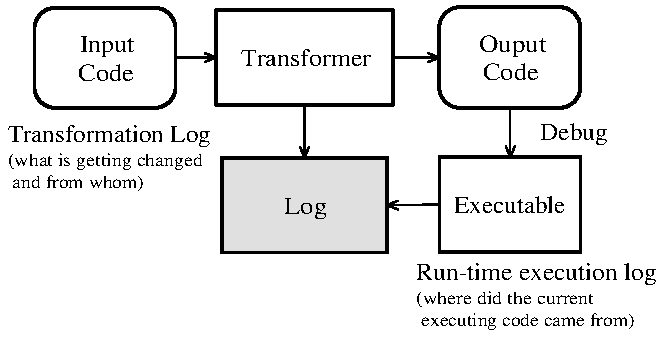
\includegraphics[width=10cm,height=!]{ch04/log}
	\caption{Transformation and Execution Log}
	\label{fig:ch04log}
\end{figure}

Traceability is integrated in the Tango framework (\fig{fig:ch04log}), and is implemented with the help of the inner attributes. Tango distinguishes between (a) transformation time log and (b) run-time execution log. The transformation log gives feedback about the transformation process. The execution log helps to trace the origin of the executed code. Traceability can be turned on and off for pieces of source code of interest by using a special explicit attribute \texttt{log}, directly in source code. When present, this attribute instructs the framework to automatically add special log calls to all methods that are transformed by every Tango transformer. The log calls are decorated with special attributes, that contain the transformer names which have edited a given method. When output code is executed, the log trace statements are printed on the console, enabling the display of the exact transformation history for each executing method (an example is given in \fig{fig:mobray}). This centralized tracing capability helps to debug the transformation-related side-effects.

As discussed in \kr{ch03}, GAAST languages support the preservation of the MDA PIM architecture into the PSM, when the PSM is source code, shifting the model transformation to the language level. The structured attribute-driven transformations of this chapter further preserve the traceability of the PIM, after the PSM transformation. Inner attributes \see{sec.inner.tags} enable the association of traceability semantics with the transformed elements. The Tango framework preserves the inner attributes in the outputted code. This approach enables tracing back the origin of the code and depending on the design of the transformers\footnote{For example, MobCon \seec{ch05} transformers are additive. They never remove the original user code from the transformed components, only append to it. This ensures complete traceability when combined with the preservation of the inner attributes.} and the redundancy of the used inner attributes, it could also used to support full round-trip engineering. The preserved inner attributes do not influence the performance of the end system. The representation of the inner attributes could also be combined with specific language support for attributes, as in the case of Java 1.5 \see{when.annotate}, to directly support traceability at run-time.


\section{Automating Attribute Transformation Concerns}
\label{ch04:sec:dep}

The transformation process for interpreting the attribute-based DSA was modularized in \sr{sec.attribute.trans} based on the domain assets. Several transformation related issues, e.g., checking for the right usage of attributes, or validating the AST to conform to the decorated attributes, must still be implemented separately in each transformer. There are many repetitive transformation concerns that crosscut more than one attribute-driven transformation. The repetite transformation concerns can be factored out from the individual $\Phi_i$ transformers, and implemented as generic attribute-driven operations $\Delta_j(\{\tau(\pi)\}, \{C\})$.  The equation~\ref{eq.par} becomes \ref{eq.ccc1}, with the $\Phi_i$-s simplified by the $\Delta_j$-s. 

\begin{equation}
\{\Gamma\} = (\bigcirc, ||)[\Delta_j(\{\tau(\pi)\}, \{C\}), \Phi_i(\phi_i, I_i, \{C_i\})]
\label{eq.ccc1}
\end{equation}

\noindent The transformation cross-cutting concerns $\Delta_j$ are candidates to be handled automatically by an attribute-driven transformation framework. For example, logging \see{sec.tango.trace} is a cross-cutting concern handled automatically by the Tango framework as part of the traceability. This section demonstrates a generic technique that can help to factor out declaratively the cross-cutting functionality $\Delta_j$, outside of the individual $\Phi_i$ transformers. To illustrate the concept, two examples of cross-cutting attribute transformation concerns are considered next.

\textbf{ I) Attribute dependencies.} In \sr{sec:var.dsa}, an example of how a web service can be modeled with DSA was given. \fig{fig:webservice-dsl} is repeated here for convenience as \fig{fig:webservice-dsl-2}. \Sr{c2.sec.dsa.attributes} illustrated how the same web service DSA can be modeled with attributes in \fig{fig:webservice}, repeated here as \fig{fig:webservice-2}.

\begin{figure}[ht]
\begin{minipage}[t]{0.4\linewidth}
\begin{center}
\begin{scriptsize}
\begin{lstlisting}[numbers=left,language=Java,frame=leftline]{}
webservice TravelAgent {
  ...
  webmethod GetHotels(){...}
  ...
}
\end{lstlisting}
\end{scriptsize}
\vspace{0.7cm}
\end{center}
\caption{A Domain-specific Extension to Implement Web Services (\fig{fig:webservice-dsl})}
\label{fig:webservice-dsl-2}\end{minipage}\hspace{1cm}%
\begin{minipage}[t]{0.4\linewidth}
\begin{center}
\begin{scriptsize}
\begin{lstlisting}[numbers=left,language=Java,frame=leftline]{}
[WebService]
class TravelAgent {
  ...
  [WebMethod]
  public void GetHotels(){...}
  ...
}
\end{lstlisting}
\end{scriptsize}
\end{center}
\caption{A Web Service Class with two Inter-depended Attributes (\fig{fig:webservice})}
\label{fig:webservice-2}\end{minipage}
\end{figure}

When a DSL (or EDSL) is used, an explicit grammar rule, such as, \texttt{web\-ser\-vi\-ce := web\-me\-thod+}, explicitly defines the context relation between \texttt{web\-ser\-vi\-ce} and \texttt{webme\-thod} in \fig{fig:webservice-dsl-2}. 
A web method will appear only inside a web service and vice-versa, a web service will contain web methods. This grammar rule is automatically enforced by the parser.
 
When attribute-based DSA are used, there is no default way how such a generic dependency constrain can be declared and enforced. It remains the responsibility of the corresponding attribute transformer to validate the dependency constrain. Depending on whether the class or its methods are considered, there are two constrains that need to be enforced: (a) public methods of a class decorated with \texttt{[Web\-Servi\-ce]} should be decorated with the \texttt{[Web\-Method]} attribute\footnote{For simplicity, it is assumed that all public methods need to be decorated. The actual implementation explained in \sr{sec:adc} removes this restriction by enabling user-defined filters for specifying which code elements, in this case methods, will be checked and which will be not.}, (b) any method decorated with a \texttt{[Web\-Method]} attribute should be declared within a class decorated with the \texttt{[Web\-Servi\-ce]} attribute. That is, the two attributes are inter-dependent. The dependency relation needs not to be symmetric, e.g., a \texttt{[Va\-li\-da\-te]} attribute may require another \texttt{[Va\-li\-da\-te.Max\-Va\-lue]} attribute, whereas the \texttt{[Va\-li\-da\-te.Max\-Va\-lue]} attribute may also be used alone.

Checking attribute dependencies is needed in any attribute family transformer, in order to make sure, for example, that suitable sub-attributes have been used. The code required to enforce dependencies between attributes, stating, for example, that a certain attribute is present in the program hierarchy before another attribute can be used, is a cross-cutting concern (CCC) that is repeated in every transformer.

\textbf{II) Virtual instances and \texttt{this} keyword usage.} This example is motivated by the implementation restrictions of the EJB \cite{www.ejb} programming model. The EJB specification states, among other restrictions, that components whose instances are managed as \textit{virtual instances} \cite{server.patterns.02} should not pass \textit{this} as a parameter or as method return value. The underlying rationale is that it makes no sense to return a direct pointer to an object that will be reused with a different internal state, at a later point of time, by the container. While the EJB implementations up to version 2.1 do not rely on attributes, Java 1.5 annotations will be used in EJB 3.0 \cite{ejb30} instead of the marking interfaces \see{attributes}.

\begin{figure}[ht]
	\begin{center}
	\begin{minipage}{5cm}
	\begin{scriptsize}
\begin{lstlisting}[numbers=left,language=Java,frame=leftline]{}
[VirtualInstance]
class C {
  ...
  [InitInstance]
  public C initialize(Id id){...}
  ...
}
\end{lstlisting}
\end{scriptsize}
\end{minipage}
\end{center}
\caption{A Class that Requires Virtual Instance Support}
\label{fig:vinstance}
\end{figure}

The imaginary example shown in \fig{fig:vinstance} supposes that the lifetime of an instance of a class \texttt{C} is going to be managed by the container, only when the class declaration is decorated with the attribute \texttt{[Vir\-tual\-Insta\-nce]}. For a class \texttt{C} tagged with the attribute \texttt{[Vir\-tual\-Insta\-nce]}, the restriction about \textit{this} must hold. The method \texttt{initialize()} of class \texttt{C} is invoked by the container when a virtual instance needs to be initialized. This method is identified by annotating it with an \texttt{[Init\-Instan\-ce]} attribute to distinguish it for later processing.

The transformer of the \texttt{[Vir\-tualInsta\-nce]} attribute needs to check the \textit{no-this} restriction for the methods that the class contains. The same check could be repeated in the member constructor transformer for the \texttt{initialize()} method, which processes the \texttt{[Init\-Instan\-ce]} attribute. Transformers for other domain assets, e.g., database connection pooling transformers, may also need to check the \textit{no-this} restriction. The same validation code needs to be repeated in different transformers for the AST blocks inside a method.

\subsection{Expressing Cross-Cutting Concerns with Meta-Attributes}

In a GAAST language \see{sec:gaast}, all entities can be decorated with attributes. \textit{Meta-attributes} are attributes used to decorate other attributes. Meta-attributes can be used to associate arbitrary semantics with attributes that can be checked for, or enforced automatically. Meta-attributes do not decorate attribute instantiation\footnote{Attribute parameters \see{ch03:sec:attrib.param} are used to express the variability of the attribute instantiation.}. Rather meta-attributes decorate attribute definitions. When an attribute $\tau(\pi)$ is defined, its definition is decorated with meta-attributes $\{\mu(\mu_{\pi})\}$, where $\mu_{\pi}$ are parameters used to specialize the meta-attribute instantiation. 
%
Meta-attributes provide a native mechanism to declaratively model the transformation cross-cutting concerns in GAAST languages. Meta-attributes help to factor the code that handles the cross-cutting concerns out of individual transformers, in generic concern processing tools, which can be made part of an attribute-driven transformation framework. The generic $\Delta_j$ transformers, working over meta-attributes $\{\mu(\mu_{\pi})\}$, can be expressed as in equation~\ref{eq.delta}. The $\{\mu(\mu_{\pi})\}$ define semantic constrains (or operations) that must hold over $\{\tau(\pi)\}$, when $\{\tau(\pi)\}$ are applied to $\{C\}$.

\begin{equation}
\Delta_j \rightarrow \Delta_j([\{\mu(\mu_{\pi})\},\{\tau(\pi)\}], \{C\})
\label{eq.delta}
\end{equation}

Using custom meta-attributes in .NET \cite{www.dotnet} is similar to using the predefined \texttt{[Sy\-stem.\-Attri\-bu\-te\-Usa\-ge\-Attri\-bu\-te]}. This special attribute is used in .NET to decorate the definition of a custom attribute, providing information about the lexical scope in which the attribute at hand can be used. Based on the usage attributes, every time a custom attribute is encountered in a program, the compiler can check whether the attribute is being used in the right lexical context, and report an error when this is not the case. The idea underlying \texttt{[Sy\-stem.\-Attri\-bu\-te\-Usa\-ge\-Attri\-bu\-te]} can be adopted to introduce new custom checks by using custom meta-attributes. 

\begin{figure}[ht]
	\begin{center}
	\begin{minipage}{12cm}
	\begin{scriptsize}
\begin{lstlisting}[numbers=left,language=Java,frame=leftline]{}
[AttributeUsage(AttributeTargets.Class)]
class NoThis : System.Attribute { ... }

[NoThis]
[AttributeUsage(AttributeTargets.Class)]
class VirtualInstance : System.Attribute { ... }

[NoThis]
[AttributeUsage(AttributeTargets.Method)]
class InitInstance : System.Attribute { ... }
\end{lstlisting}
\end{scriptsize}
\end{minipage}
\end{center}
\caption{Modeling \texttt{[NoThis]} Constraint as a Meta-Attribute}
\label{fig:no-this}
\end{figure}

Consider for example, the \textit{no-this} restriction \see{ch04:sec:dep} modeled as a \texttt{[No\-This]} me\-ta-attri\-bu\-te. The \texttt{[No\-This]} meta-attribute is used to decorate the definition of all attributes that need to check, or enforce, the \textit{no-this} constrain, as shown in the .NET C\# example of \fig{fig:no-this}. A cross-cutting attribute checker tool, that enforces the \textit{no-this} restriction, needs to check each attribute of a code entity, whether the attribute definition\footnote{Whether the attributes of the attribute itself.} contains a \texttt{[No\-This]} (meta-) attribute. If the condition is fulfilled, then the methods decorated with the corresponding attribute need to be checked. The cross-cutting concern checker tools operate outside the $\Phi_i$ transformers, reducing the amount of code that needs to be implemented and debugged in each individual $\Phi_i$ transformer.

The \textit{attribute dependency} example \see{ch04:sec:dep} is more complex, as it requires a bigger context to be handled, when the attribute dependencies are resolved. Ideally, it is preferable to declare the attribute dependencies similarly to grammar rules. Meta-attributes enable expressing attribute dependencies declaratively in GAAST languages. The rest of this section explores in detail how attribute dependencies can be modeled as meta-attributes and how they can be enforced automatically. The presented implementation is based on .NET \cite{www.dotnet}. The details of the attribute processing in .NET were discussed in \sr{c3.sec.dnet}.

Using meta-attributes frees the developers that write attribute-driven transformers from coding repeated concerns, by centralizing the way cross-cutting concerns are processed. The developers only declare constrains, e.g., dependencies, without taking explicitly care of how the corresponding concerns are resolved and enforced. 
There are of course many ways \see{sec.c4.related} to declare and enforce architectural dependencies \cite{minsky.98}. Using meta-attributes to decorate other attributes is a natural way for GAAST-like languages, because meta-attributes could be directly processed by the attribute-driven transformers presented in this chapter. 

\subsection{The Attribute Dependency Model}
\label{sec:model}

The attribute dependency model presented in this section distinguishes between (a) \textit{required} dependencies, stating that a given attribute requires another one in order to be used, and (b) \textit{disallowed} dependencies, stating that a given attribute cannot be used, if another attribute is present. 
Furthermore, children nodes in a program's structural hierarchy can declare dependency constrains on parents of any level, and vice-versa. 
An attribute of a certain program element instance may require that certain attributes are present in the set of the attributes of the structural children of its program element. For example, an attribute of a $Class$ may require that a certain attribute be present in the annotation of the class' $Methods$. The attribute dependency model generalizes these notions to any depth of the structural tree. %The reverse is also true. An attribute of a child structural element instance may require a certain attribute to be present in the set of the attributes specified for the parent instance. 

A restriction in this model is that the attributes of a program element instance cannot place any constraint on the attributes of sibling instances. For example, the attributes that a $Field$ instance is decorated with, cannot imply anything about the attributes of $Method$ instances, or attributes of other $Field$ instances. In the prototype for the J2ME MIDP \seec{ch05} sibling dependences are not used. However, the attributes of a program element instance can place constrains on the other attributes of the same instance. For example, a method attribute $a_{m1}$ of a method $m$ may require that another attribute $a_{m2}$ to be present for $m$. A more generic dependency model could be created (to include siblings constrains), but the more detailed semantics add nothing new to the meta-attribute concepts discussed.

The semantics of the $disallowed$ relation on the structural AST elements and instances can be specified similarly and will not be repeated.

\subsection{The \texttt{[DependencyAttribute]} Class}

.NET custom attributes are classes derived from the class \texttt{Sy\-stem.Attri\-bu\-te} \see{c3.sec.dnet}. Custom attributes may have arguments specified either as constructor parameters (unnamed arguments), or as properties of the attribute class, which generate \textit{getter} and \textit{setter} methods in C\# (named arguments). Attribute classes may also contain methods and state (instance fields), as every other .NET class does.
Using properties to specify attribute arguments is more flexible than using constructors, because .NET does not support complex types to be passed as parameters to the constructors\footnote{Only basic constant types and \texttt{Sy\-stem.Ty\-pe} can be used. \texttt{Sy\-stem.\-Object} is also listed in the documentation, because it is the parent of simple types and of \texttt{Sy\-stem.Ty\-pe}. This does not mean that arbitrary objects can be passed as constructor parameters.}. 

To handle the attribute dependencies, a new meta-attribute named  \texttt{De\-pen\-dency\-Attri\-bu\-te}\footnote{When used in code the suffix \texttt{Attri\-bu\-te} may be omitted from the name of an attribute class.} is defined as a custom attribute class. The \texttt{De\-pen\-dency\-Attri\-bu\-te} contains one \texttt{Re\-quired*} and one \texttt{Dis\-allowed*} property for every program element type, for which the attribute dependency checking is supported (\texttt{Assembly}\footnote{A .NET \texttt{Assembly} maps roughly to a Java JAR file. The \texttt{Assembly} attributes map roughly to custom JAR manifest entries.}, \texttt{Class}, \texttt{Me\-thod}), as shown in \fig{fig:da}. 
Given that the number of the node types in a program's structural tree is limited, it makes sense to enumerate such operations. This makes the code easier to understand compared to having a single dependency property for all meta-element types.

\begin{figure}[ht]
\begin{center}
\begin{minipage}{10cm}
\begin{scriptsize}
\begin{lstlisting}[numbers=left,language=Java,frame=leftline]{}
[AttributeUsage(AttributeTargets.Class)]
public class DependencyAttribute : System.Attribute {
  ...
  public DependencyAttribute() {...}
  public Type[] RequiredAssemblyAttributes {...}
  public Type[] DisallowedAssemblyAttributes {...}
  public Type[] RequiredClassAttributes {...}
  public Type[] DisallowedClassAttributes	{...}
  public Type[] RequiredMethodAttributes {...}
  public Type[] DisallowedMethodAttributes {...}
}
\end{lstlisting}
\end{scriptsize}
\end{minipage}
\end{center}
\caption{The Dependency Attribute}
\label{fig:da}
\end{figure}

Adding support for object \texttt{Fields} to this model is trivial \see{sec:adc}. Readers familiar with .NET may note that \texttt{na\-me\-spa\-ces}\footnote{A .NET \texttt{na\-me\-spa\-ce} maps roughly to a Java  \texttt{package}.} were skipped from the list of program elements above. The reason is that a \texttt{na\-me\-spa\-ce} is a logical, rather than a physical concept, so even though theoretically a \texttt{na\-me\-spa\-ce} can be decorated with attributes, practically there is not a single physical place where to store the attributes, given that a \texttt{na\-me\-spa\-ce} may extend in many modules and assemblies\footnote{This is the reason why .NET does not list \texttt{na\-me\-spa\-ce} as an entry in the \texttt{Attri\-bu\-te\-Tar\-gets} enumeration.}.

The current .NET implementation seems to restrict the complexity of the validation logic that could be implemented inside the property methods of a custom attribute. 
The .NET documentation is not clear about whether that code is ever activated. Furthermore, if the code inside a property is more than a simple assignment, that property may be not included in the attribute class without any warning from the C\# compiler.
For this reason, the code of the \texttt{De\-pen\-den\-cy\-Attri\-bu\-te} properties must be kept as simple as possible, and checks that could normally be done by the property method code, e.g., that the attributes passed as a parameter to a property have the right \texttt{[Sy\-stem.Attri\-bu\-te\-Usa\-ge\-Attri\-bu\-te]} target\footnote{E.g., that \texttt{Attri\-bu\-te\-Tar\-gets.\-Me\-thod} is present in the declaration of an attribute included in the list \texttt{Re\-qui\-red\-Me\-thod\-Attri\-bu\-tes}.}, should be postponed until the actual dependency checking is performed.

The \texttt{De\-pen\-den\-cy\-Attri\-bu\-te} only stores the required / disallowed attribute arrays (lists), and contains only code for printing these arrays as strings, needed for error and log reporting. It does not contain any code to interpret the dependencies and its implementation has no other module dependencies. As a consequence, the \texttt{De\-pen\-den\-cy\-Attri\-bu\-te} is independent of any particular dependency checker implementation and can be distributed and used alone to decorate attribute libraries. 

%\subsubsection{Using the Dependency Attribute}

\begin{figure}[ht]
\begin{center}
\begin{minipage}{12cm}
\begin{scriptsize}
\begin{lstlisting}[numbers=left,language=Java,frame=leftline]{}
[Dependency(RequiredMethodAttributes(new Type[]{typeof(WebMethod)})]
[AttributeUsage(AttributeTargets.Class)]
class WebService : System.Attribute { ... }

[Dependency(RequiredClassAttributes(new Type[]{typeof(WebService)})]
[AttributeUsage(AttributeTargets.Method)]
class WebMethod : System.Attribute { ... }
\end{lstlisting}
\end{scriptsize}
\end{minipage}
\end{center}
\caption{Using the Dependency Attribute}
\label{fig:code1}
\end{figure}

\fig{fig:code1} shows how the \texttt{De\-pen\-den\-cy\-Attri\-bu\-te} is used in code to express the dependency semantics of the attributes \texttt{[WebService]} and \texttt{[WebMethod]}, for the example of \fig{fig:webservice-2}. The C\# '\texttt{typeof}' operator is used to obtain an instance of the class type of each attribute. Class types fall into the category of types supported by .NET as attribute property arguments. The dependency lists are saved as C\# arrays inside the two instances of the  \texttt{De\-pen\-den\-cy\-Attri\-bu\-te} and will be preserved from .NET as part of the IL binary meta-data.

\subsection{The Attribute Dependency Checker (ADC) Tool}
\label{sec:adc}

The Attribute Dependency Checker (ADC) tool is implemented as a \textit{post-processor} using the .NET \texttt{Reflection API}, exploring the reflective capabilities of GAAST languages \see{sec:gaast}. After the code is compiled and linked, the ADC tool can be run over the IL binaries, to detect the possible attribute dependency errors. Alternatively, ADC could be implemented as a \textit{pre-processor} tool to be run before the source is compiled, using the \texttt{Code\-Dom API}\footnote{A third-party implementation of \texttt{ICo\-de\-Pa\-rser} for C\# can be found in \cite{cs.codedom.parser}.}.

\fig{fig:implementation} shows the architecture of the ADC tool. Almost all the functionality of the dependency checker is found in the abstract class \texttt{Attri\-buteDe\-pe\-nde\-ncyChe\-cker}. This class uses several other helper classes and interfaces (a) to  filter the processed elements (\texttt{IDe\-pende\-ncyFi\-lter}), (b) to log information about the progress of the checking process (\texttt{IChe\-ckLo\-gger}), and (c) to report errors (\texttt{Error\-Re\-port}). The \texttt{ICo\-ntextMap} class encapsulates the meta-model structure in a single place using a special internal coding. The ADC tool can be invoked from the command-line, or programmatically. 
For illustration, \fig{fig:using} shows how the ADC library can be used programmatically to check the attribute dependency constrains for all elements of a given .NET assembly (line 1). 

\begin{figure}[ht]
	\begin{center}
		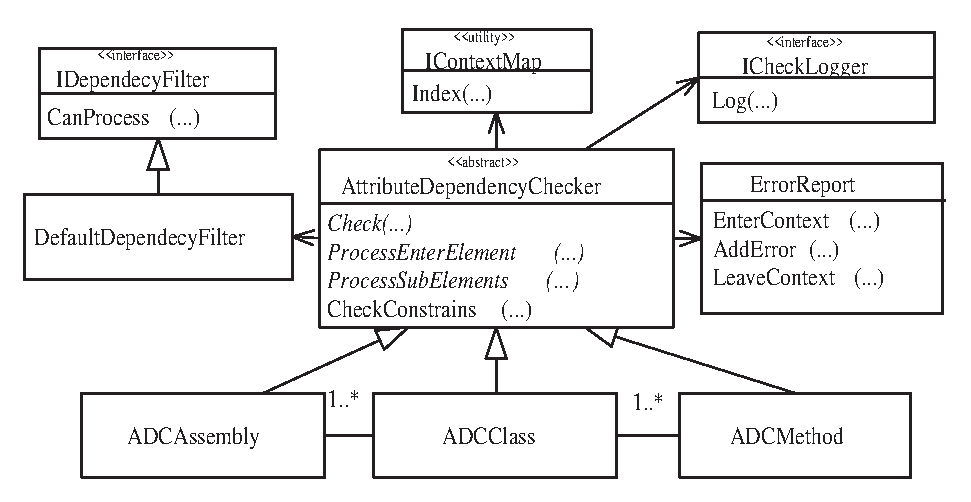
\includegraphics[width=12cm,height=!]{ch04b/implementation2}
	\end{center}
	\caption{The Run-time Attribute Dependency Checker Structure}
	\label{fig:implementation}
\end{figure}

\begin{figure}[ht]
\begin{center}
\begin{minipage}{7cm}
	\begin{scriptsize}
\begin{lstlisting}[numbers=left,language=Java,frame=leftline]{}
Assembly a = ...; // obtain an assembly
ADCAssembly c = new ADCAssembly();
c.Filter = ...;   // set filter
c.Logger = ...;   // set logger
c.Check(a);       // check the assembly
if(c.errors.HasWarnings())
{ // process: c.errors.GetWarnings() ... }
if(c.errors.HasErrors())
{ // process: c.errors.GetErrors() ... }
\end{lstlisting}
  \end{scriptsize}
\end{minipage}
\end{center}
  \caption{Using the Run-time Attribute Dependency Checker in Code}
	\label{fig:using}
 \end{figure}

In order to implement the semantics of the dependency attribute, initially the attribute dependency sets need to be built for every structural element, by processing the element and all its structural children. After the dependency sets are constructed, the dependency constrains of the element can be checked. That is, a post-order transversal of the structural tree is required. A boolean flag in \texttt{Attri\-bute\-De\-pen\-de\-ncy\-Che\-cker} controls whether the inherited attributes of the structural elements are processed or not. 
The actions performed during a call to the \texttt{Check(t)} method (line 5 in \fig{fig:using}), where \texttt{t} is the current program element whose attribute dependencies are being checked for, are illustrated in \fig{fig:seq-diag}. 

\begin{figure}[ht]
	\begin{center}
		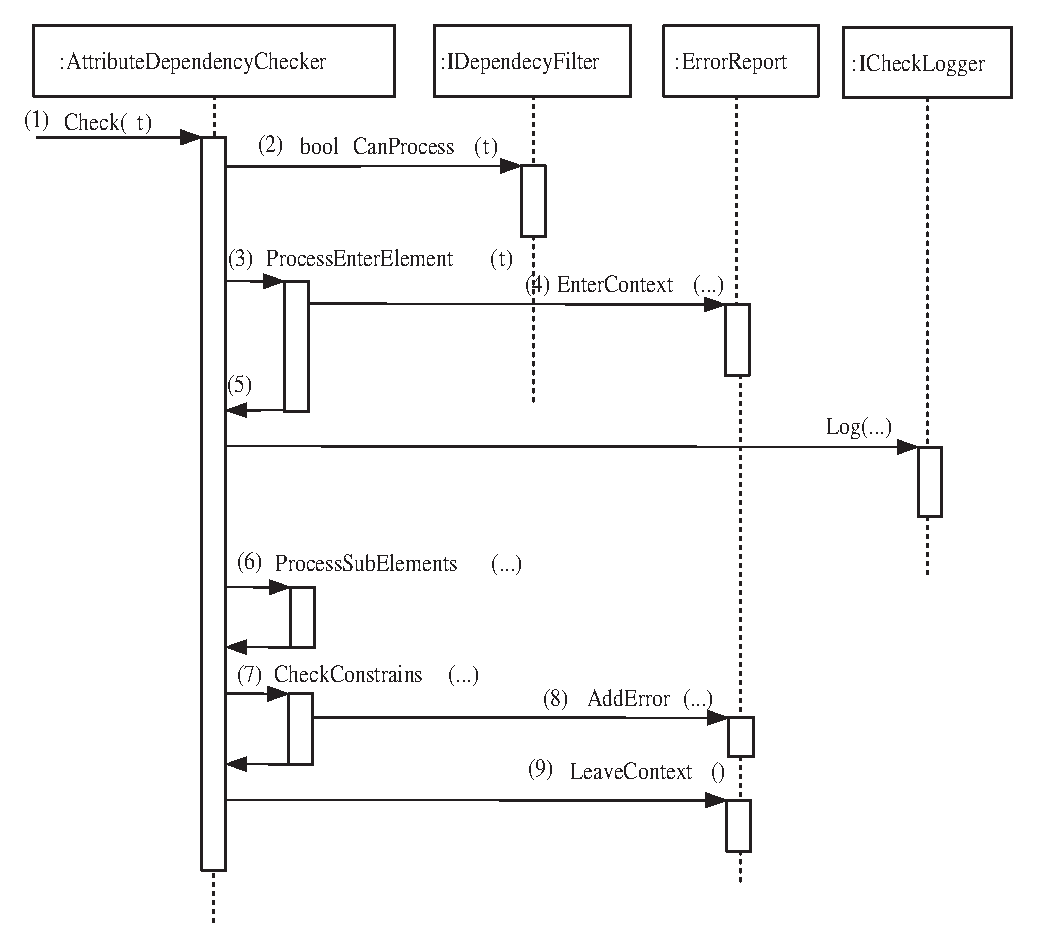
\includegraphics[width=12cm,height=!]{ch04b/seq-diag}
	\end{center}
	\caption{UML Sequential Diagram of \texttt{Check()} Method Call}
	\label{fig:seq-diag}
\end{figure}

First, the filter object is used to check whether the element at hand should be processed (step 2 in \fig{fig:seq-diag}). 
Filters can be used to put arbitrary constraints on the elements that will be processed, e.g., by using pattern matching on names. The \texttt{De\-fault\-De\-pen\-de\-ncyFi\-lter} processes all the elements. 
The ADC command-line tool uses a customized filter called \texttt{Class\-De\-pen\-de\-ncyFi\-lter} derived from \texttt{De\-faultDe\-pen\-de\-ncyFi\-lter} that can restrict checking to a subset of classes, whose names are given in the command-line. More sophisticated filters can be written and used programmatically (line 3 in \fig{fig:using}). Filters can also be used to implement profiling by keeping track of various counters; e.g., \texttt{Class\-De\-pen\-de\-ncyFi\-lter} counts the number of classes and the methods processed.

Next, the call to \texttt{Process\-Enter\-Element()} (step 3) sets the proper \texttt{Error\-Report} context (explained later) in step 4, which is used when processing the sub-elements of the element at hand. The \texttt{Process\-Sub\-Ele\-ments()} method in step 6 calls the \texttt{Check()} method of all sub-elements. As shown in \fig{fig:implementation}, the specific attribute checkers for different meta-elements, e.g., \texttt{ADC\-Assembly} and \texttt{ADCClass}, are derived from \texttt{Attri\-bute\-Depe\-ndency\-Che\-cker} by implementing the abstract methods: \texttt{Check(object t)}, \texttt{Pro\-cess\-EnterEle\-ment(object t)}, and \texttt{Pro\-cess\-Sub\-Ele\-ments(ref Array\-List ctx,\- object t)}.
For illustration, \fig{fig:proc-sub-impl} shows the implementation of the \texttt{Pro\-cess\-Sub\-Ele\-ments} method in \texttt{ADC\-Class}. Only the traversal functionality for finding the sub-elements is part of this method.

\begin{figure}[ht]
\begin{center}
\begin{minipage}{12cm}
	\begin{scriptsize}
\begin{lstlisting}[numbers=left,language=Java,frame=leftline]{}
protected override void ProcessSubElements(ref ArrayList ctx, object t) {
  MethodInfo[] m = ((Type)t).GetMethods(
    BindingFlags.Instance |
    BindingFlags.Public |
    BindingFlags.DeclaredOnly |
    BindingFlags.NonPublic);

  foreach(MethodInfo mi in m) {
    ADCMethod adc = new ADCMethod();
    CopyStateTo(adc);
    adc.InitialContext = ctx;
    adc.Check(mi);
  }
}
\end{lstlisting}
  \end{scriptsize}
\end{minipage}
\end{center}
  \caption{\texttt{ADCClass} Implementation of \texttt{ProcessSubElements} Method}
	\label{fig:proc-sub-impl}
 \end{figure}

The context to be used during the processing of a node and its descendants (the parameter \texttt{ctx} in the signature of \texttt{Pro\-cess\-Sub\-Ele\-ments}) is managed as an \texttt{Array\-List}, similarly to the method call stack frames in a compiler \cite{aho.88}.
A frame in the context array contains the attributes and the dependency attributes of a particular element. As the structural tree is traversed by calling \texttt{Pro\-cess\-Sub\-Ele\-ments}, the dependencies context is filled by passing the \texttt{ctx} object to every processed sub-element. When being processed, an element can modify the dependency information of the context frames of its parents.
%After a sub-element has been processed, its frame is removed (pop up) from the context.
After all sub-elements of a given element are processed, all the required context information is in the context stack frames. This information can be used to check the dependencies of the given element. The dependency meta-attributes of the current attribute are compared with the total dependency attributes for the current frame, using set operations in the \texttt{Check\-Con\-strains()} method (step 7 in \fig{fig:seq-diag}).
 
The \texttt{:Error\-Re\-port} object maintains its own separate context stack (set up in step 4), so that when an error is reported in step 8, the error message can be embedded within the proper structural context. The \texttt{Error\-Re\-port} context is used to report messages in a useful way, as illustrated by the error message:

\begin{scriptsize}
\begin{verbatim}
| Required CLASS attribute missing:
| adctests.CA01Attribute @ adctests->adctests.nunit.TDependencyUtils
\end{verbatim}
\end{scriptsize}

\noindent This error message specifies that the required class attribute \texttt{adc\-tests.CA01\-Attri\-bu\-te} is missing in the class \texttt{adc\-tests.nunit.TDe\-pe\-ndency\-Utils}, which is part of the \texttt{adctests} assembly.
%
By default \texttt{Error\-Re\-port} accumulates the errors, but this behavior can be changed via a switch, so that it will stop the checker execution when an error happens, by throwing a \texttt{ADC\-Excep\-tion}. The \texttt{Error\-Re\-port} contains also functionality to accumulate, or immediately report, the improper usages in code of the parameters passed to the \texttt{De\-pe\-ndency\-Attri\-bu\-te} itself. An example is passing an attribute declared with a class lexical scope, as an argument to a \texttt{Re\-quired\-Me\-thod\-Attri\-bu\-te} property.

Finally, the \texttt{ICheck\-Logger} interface (step 5) enables the programmer to associate a custom output stream logger with the dependency checker (line 4 in \fig{fig:using}). If the logger stream is not \texttt{null}, a hierarchy of the processed elements with details about their attri\-bu\-tes and attri\-bu\-te dependencies is printed in the logger stream. A filter could also be used for custom logging. All objects shown in \fig{fig:seq-diag}, with exception to the  \texttt{:Attri\-bu\-te\-De\-pende\-cyChe\-cker}, are singletons and are passed to the processing of the sub-elements as part of the context. 

The implementation of the class \texttt{Attri\-bu\-te\-De\-pe\-ndency\-Che\-cker} is generic with regard to the implementation of both the \texttt{De\-pe\-ndency\-Attri\-bu\-te} and the meta-model elements. This means that the implementation of the \texttt{Attri\-bu\-te\-De\-pe\-ndency\-Che\-cker} class can be reused with new attributes as well as with other meta-model elements. The \texttt{Attri\-bu\-te\-De\-pe\-ndency\-Che\-cker} achieves this generality by using a combination of the following three techniques:

\begin{itemize}

\item First, all the hierarchy information of the supported meta-model is factored out into two static methods of the \texttt{ICon\-text\-Map} utility class. \texttt{Attri\-bu\-te\-De\-pe\-nden\-cy\-Che\-cker} uses the \texttt{ICon\-text\-Map} to implement a strategy pattern \cite{dpatterns}. By changing the \texttt{ICon\-text\-Map} class, users can change the supported meta-model. Theoretically, the information in the \texttt{ICon\-text\-Map} is enough to check the dependencies, i.e., no specific checker classes for different elements of the meta-model, e.g., \texttt{ADC\-Class} would be needed. However, the .NET Reflection API design is not consistent for traversing the meta-elements hierarchy. Other API-s, e.g., XML DOM \cite{mcl.01}, have a single base interface\footnote{The \texttt{Node} interface in XML DOM.}, from which all elements are derived. .NET Reflection API does not expose a single generic interface for all meta-element types, because the number of meta-elements is limited. This requires that when adding new meta-elements to the ADC library, special classes need to be derived for the new elements. These new classes will contain only code to traverse the sub-elements, as described above (\fig{fig:proc-sub-impl}).

\item Second, given that the structure information of the meta-model is present in the \texttt{De\-penden\-cyAttri\-bute} property names, the reflection inside the \texttt{Check(...)} method is used over the \texttt{De\-pende\-ncyAttri\-bute} properties, to map them to the internal \texttt{ICon\-text\-Map} data. The use of the reflection ensures that if the required / disallowed properties of the \texttt{Depe\-nde\-ncy\-Attri\-bute} class are added or removed, the implementation of the \texttt{Attri\-buteDepen\-dencyChe\-cker} does not need to be changed. Another generic alternative would be to generate the checker code based on the \texttt{Depen\-dency\-Attri\-bute} implementation, but this would require to re-generate and re-compile the \texttt{Attri\-buteDepen\-dencyChe\-cker} class for every different version of the \texttt{Depen\-dency\-Attri\-bute} implementation.

\item Third, the template method pattern \cite{dpatterns} is used to call abstract methods that need to be implemented in the derived classes, such as the \texttt{Proce\-ssSubEle\-ments} method in \fig{fig:proc-sub-impl}, required to traverse the sub-elements. The entire checking functionality is part of the abstract class \texttt{Attri\-buteDe\-pende\-ncyChe\-cker}.

\end{itemize}

The resulting ADC library can be easily extended to support new meta-elements. If a new type of checker for attributes of another meta-element need to be added, then a class from \texttt{Attri\-bu\-te\-De\-pe\-ndency\-Che\-cker} must be derived. The derived class implements the abstract methods discussed above. In addition, the \texttt{ICon\-text\-Map} class needs to be modified to accommodate the hierarchical structural relation of the new element, with regard to the existing elements. 

\section{Related Work}
\label{sec.c4.related}

%Attribute transformations techniques presented in this chapter are specialized for the interpretation of attribute-based DSA required in mobile product-lines. The vertical and horizontal modularization techniques are made possible only by exploring the characteristic of this specific domain and the hardwired language meta-model. The specific modularizations would not have been possible if attribute transformations were addressed from a more generic level.

Attributes are a form of graph labeling \cite{term.rewrite,Plump.95,mens.99}. Attributes make it possible to associate arbitrary semantics with graph nodes of interest, and can be used to drive graph transformations. Considering attributes in a very generic level is not very useful in practice. For example, being able to normalize a series of add / remove / modify operations applied to a graph \cite{mens.99} is an interesting theoretical operation. In the domain of mobile applications considered as a use case in this book, the scenarios that add the same block of code or method, or remove it several times, do not happen. Graph labeling is more interesting when it is specialized for a domain. For example, in \cite{Biggerstaff.ICRS6} tags are used to reduce transformation search space \cite{ptm.03} by serving as transformation hints, in the same way as tags in MDA \cite{mda.frankel} models. The class of graph labels addressed in this book is made of attributes used directly at the programming language level. Attributes are complex graph labels that are specialized using parameters, contain behavior, and could be decorated themselves with other attributes.

Several general-purpose languages, such as .NET \cite{www.dotnet} and Java 1.5 \cite{www.java.attrib.04}, already offer support for attributes. As discussed in \kr{ch03}, these languages offer also GAAST-like means to process the code decorated with attributes. Other non-mainstream approaches also exists \cite{java.explicit.programming,java.attrib4j}. These approaches fall in the category of API-based generators \cite{voelter.generation,generative.00}. The GAAST-level of generality was the starting point for the modularization techniques presented in this chapter. The parsing issues were not addressed on purpose in Tango, to provide flexibility to use any GAAST API, or meta-programming tool discussed in \sr{sec.meta.prog}, e.g., \cite{java.openJava,batory98jts,java.jse,java.epp,java.maya,qdox} to map the AST to the common Tango OO model.

Tango modularization techniques can be seen as domain specialization of graph rewriting systems \cite{term.rewrite,Nagl:96,mens.99}. The changes introduced by an attribute-driven transformer to an annotated class could be seen as a series of primitive operations. Tango supports a hardwired language meta-model with a finite number of elements. This makes it possible to enumerate the edit operations. The approach is similar to implementing graph-based schema evolutions \cite{Banerjee.87}, but specialized for a special set of OO attribute-driven transformers.

Stratego \cite{stratego.01,ptm.03} is a library of strategy operators and traversal primitives to reduce the program transformation costs. Stratego is implemented as a set of reusable transformations primitives that can be used with any language system, given that a suitable parser to map the specific language constructs, to Stratego constructs can be created. The Stratego modules are translated to C code. Stratego organizes transformation operations as series of strategies that work over grammar rules, to support, for example, term rewriting \cite{term.rewrite}. \textit{"A strategy is an operation that transforms a term into another term or fails"} \cite{stratego.01}. A strategy is made up of:
\begin{itemize}
\item \textit{Traversal primitives} that support reusable term traversal techniques. Examples: \textit{all} - all nodes in an expression; \textit{repeat} - an generic iteration strategy to repeat an operation; \textit{bottomup} - does a bottom-up traversal of an expression.
\item \textit{Strategy operators} that allow the combination of strategies. Examples: \textit{sequential composition} - combines a sequence of  traversal primitives; \textit{choice} - selects between two or more traversal primitives. 
\end{itemize}

\noindent The approach presented in Tango is different in two ways from Stratego: (a) the strategies are organized in layers and (b) the strategies are specialized for the entities of each layer.

There are several general-purpose transformation frameworks, e.g., DMS \cite{dms.02}, TXL \cite{txl.04} and ASF+SDF \cite{asfsdf.02}, which can be used to address domain-specific transformations. These general-purpose frameworks have an open meta-model meaning that any specific language can be mapped to them. These tools could also be used to process explicit attributes. However, generic frameworks do not provide declarative specialized rules for every specific domain of interest. Hardwiring the domain, as in Tango, enables abstracting the transformation strategy operations at different levels. 

Tango's vertical attribute modularization bears resemblance to layered context-sensitive graph grammars \cite{Rekers-Schuerr02:97} and multi-stage programming \cite{Taha.1997}. Layered grammars \cite{Rekers-Schuerr02:97} have been used to recognize left-hand side patterns in graphs, and specify an evaluation order for graph rewriting rules. Tango is specialized only for attribute-driven transformers. Multi-stage programming uses special annotations to structure the computation of expressions as multi-stage transformations. Multi-stage programming is driven by the need for optimizations and partial evaluation \cite{jonesetal.93} and uses a predefined set of annotations. Tango can be used to implement arbitrary invasive transformers \cite{java.compost} at source code level, in the top of a GAAST-like language. Tango also supports an arbitrary number of user defined attributes. 

Some transformation approaches generalize the ways a transformer works with an AST-like representation of the program: (a) \textit{Filtering related approaches}, e.g., JPath \cite{extract}, are motivated by XPATH \cite{url.xpath} node query language for XML \cite{skonnardetal.01}. The idea is to be able to define XPATH-like queries over the AST to declaratively select sets of nodes of interest. For example, the query  "\texttt{//class[@name=\-"Class1"]/\-method[@name=\-"Method1"]}" selects and returns all methods named \textit{Method1} found in class named \textit{Class1}. (b) \textit{Mapping related approaches} build upon filtering related approaches and that are motivated by XSLT \cite{xslt} and more recently by MOF Query View and Transformation \cite{mof-qvt-ibm-sub.03} proposals. These approaches define declaratively how to map a set of selected nodes to another set of nodes, enabling this way the generic transformations of one graph to another. These approaches are very general. For example, XML and XPATH are used internally in Tango to implement the specific Tango features on top of them.

The feature-based categorization of MDA transformation approaches presented in \cite{model-approach.03} distinguishes between \textit{model-to-code} and \textit{model-to-model} approaches. Tango is a \textit{code-to-code} transformation framework. Given that the transformation of a marked model to marked code is trivial \see{sec.gaast.map}, the approach can be seen also as \textit{model-to-code}. With regard to the implementation, Tango can be seen as a \textit{template}-like transformer with source-oriented deterministic iterative rules. The categorization in \cite{model-approach.03} is too wide, and many tools could fall into the same category. Tango is unique for its well-structured layers, extensibility of primitive operations, and heavy reliance on inner tags.

Code snippets in Tango are an example of the combination of template and frame-based systems \cite{generative.00,voelter.generation}. Similar approaches include syntactic unit trees \cite{majkut.03} and various template and macro-based approaches \cite{java.epp,java.jse}. Tango code snippets differ from these approaches, because code snippets are restricted to represent only non-structural elements, e.g., a block of code inside a method. Tango code snippets can also be labeled with inner tags and reprocessed later as atomic elements of the AST.

Declaring and checking attribute dependencies is one example of explicitly enforcing architectural principles \cite{minsky.98}. Attributes offer a unified way to express evolution invariants in languages that support explicit annotations, given that any structural entity can be decorated independently of the syntax. This makes attributes attractive for expressing law-governed system evolution rules. Architectural principles that must hold between program entities can be expressed as attribute dependencies between architectural attributes used to decorate program entities. System-wide invariants can be expressed in .NET as \texttt{Asse\-mbly} attributes and system-wide rules can be expressed declarative by using meta-attribute annotations over the architectural attributes.

The meta-attributes approach enables explicit factorization of cross-cuttings concerns in attribute-driven transformers. Meta-attributes make the cross-cuttings concerns definitions declarative and fit well in the paradigm of a GAAST language. Meta-attributes are not well-suited for checking arbitrary program restrictions. Cross-cuttings concerns based on meta-attributes can be factorized using specific tools, e.g., ADC \see{sec:adc} or any generic me\-ta-pro\-gramming tool. There are also generic me\-ta-pro\-gramming tools \cite{www.pmd,www.tj,XIRC} designed to ease enforcing of program rules that cannot be checked directly by the programming language compiler. These tools could be used to implement checking based on attributes directly, or based on meta-attribute factorizations if they can access them. Cross-cuttings concerns could also be factorized with AOP \cite{kiczalesetal.97,Laddad.aop,XIRC,aop.attrib.05} techniques \see{ch2:aop}. Aspect-oriented programming techniques can be also used to enforce architectural decisions. An example how AspectJ \cite{www.aspectjt} can be used to enforce system-wide constrains is given in \cite{shomrat.01}\footnote{There are meta-programs that cannot be expressed as AspectJ programs.}. 

Attribute extension grammars can be used to enforce properties about library components that can not be enforced otherwise with object-oriented systems \cite{hedin.97}. The work has been superseded by language technologies, such as .NET \cite{www.dotnet}, that directly support attributes and offer GAAST-like access to the AST information along with the decorated attributes. The meta-attributes approach enforces rules at a more abstract level, using attributes to define declarative rules that must hold between attributes.

It is also possible to define a central notion of dependency and model any kind of dependency by a Dependency Code Calculus (DCC), based on a computational lambda calculus \cite{abadi99core}. Such a formal abstraction can be interesting for proving properties of dependent system elements, but it must be specialized to a specific domain to be of real usage, yielding different special purpose calculuses \cite{abadi99core}. However, some of the dependency problems mentioned in \cite{abadi99core}, such as slicing calculus, do not map directly into source code program dependencies and cannot be expressed as source code attributes.

\cendsection{Chapter Summary}

The transformations of attribute decorated entities become problematic in a system when the number of attributes and their required interpretation context grows. The attribute-driven transformer implementation is the ultimate source of documentation about the semantics of an attribute or a set of such. It is important that the transformation process is implemented in a well structured and modular way to ease understanding and enhance reuse.

The domain knowledge for attribute-based DSA used to support mobile product-lines is explored to modularize attribute-driven transformers. The overall attribute-based DSA transformation is structured in parts corresponding to the domain assets, which are modeled as attribute families.

To enable declarative composition of the transformer units, inner attributes are used to express the inter-transformation semantics. Inner attributes serve as a uniform composition mechanism for attribute-driven transformers, that treat the inner attributes equivalently to explicit attributes. Inner attributes make the transformer coupling explicit.

The knowledge of semantics of the domain assets is used to define the transformation workflow. The process is partially automated by having the dependencies expressed as \textit{before} or \textit{after} lists. The generated dependency graph can be overwritten manually by using specialized workflow operations to resolve potential conflicts.

The hardwired OO language meta-model addressed by Tango is explored to achieve a vertical modularization of transformer units. The transformation strategy is structured according to the nesting of the structural elements in the language meta-model. This structure is enforced with language constructs. Specific strategy operations optimized for each layer are created to make the transformer implementations more declarative.

The common OO meta-model is isolated inside the transformation framework, from the details of the specific language, by using code snippets. Code snippets are parameterized templates that contain language specific syntax, and are used only inside the member constructors, e.g., the method transformers.

Repetitive cross-cutting attribute-transformation concerns are factored out of individual transformers, and made part of generic tools of the transformation framework. Meta-attributes offer a convenient way to implement a mix-ins structure, used to declaratively express the cross-cutting concerns of attribute-driven transformers.

Attribute dependencies are a cross-cutting attribute-transformation concern that is made declarative by using meta-attributes. A special tool was demonstrated, which extends .NET to declare, and automatically check, attribute dependencies using Reflection over the IL binaries. 
